\textbf{Recurrent neural network} \\[0.2em]
Con người không bắt đầu suy nghĩ từ đầu mỗi giây.
Khi bạn đọc bài luận này, bạn hiểu từng từ dựa trên sự hiểu biết của bạn về các từ trước đó.
Bạn không nên ném mọi thứ đi và bắt đầu suy nghĩ lại từ đầu. Suy nghĩ của bạn
có sự lưu lại.

Mạng lưới thần kinh truyền thống có thể làm được điều này, và nó có vẻ như là một
thiếu sót lớn.
Ví dụ, hãy tưởng tượng bạn muốn phân loại loại sự kiện nào đang diễn ra tại mọi thời điểm trong phim.
Nó không rõ làm thế nào một mạng lưới thần kinh truyền thống có thể sử dụng lý lẽ của nó về các sự kiện trước đó trong phim để thông báo cho những sự kiện sau này.

Recurrent neural network giải quyết vấn đề này. Chúng là các mạng có các vòng lặp trong đó, cho phép thông tin tồn tại.
\begin{figure}[!htb]
    \center{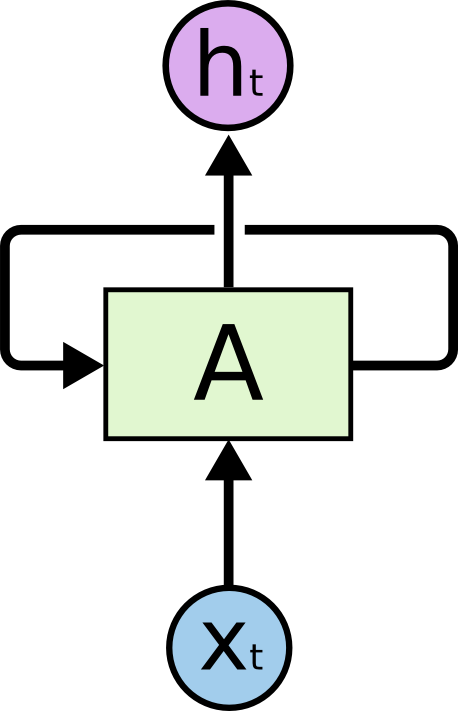
\includegraphics[width=2cm]
    {figure/model/RNN-rolled.png}}
    \caption{\label{fig:rnn-rolled} Recurrent Neural Network có vòng lặp.}
\end{figure}

Trong sơ đồ trên, một đoạn của mạng thần kinh, \(A\), xem xét một số xt đầu vào và xuất ra một giá trị
\(h_t\).Một vòng lặp cho phép thông tin được truyền từ một bước của mạng sang bước tiếp theo.

Những vòng lặp này làm cho Recurrent neural network có vẻ như bí ẩn.
Tuy nhiên, nếu bạn suy nghĩ nhiều hơn một chút, hóa ra họ không phải là một mạng lưới thần kinh bình thường.
Recurrent neural network có thể được coi là nhiều bản sao của cùng một mạng, mỗi bản tin truyền cho một người kế nhiệm.
Xem xét những gì xảy ra nếu chúng ta bỏ vòng lặp:

\begin{figure}[!htb]
    \center{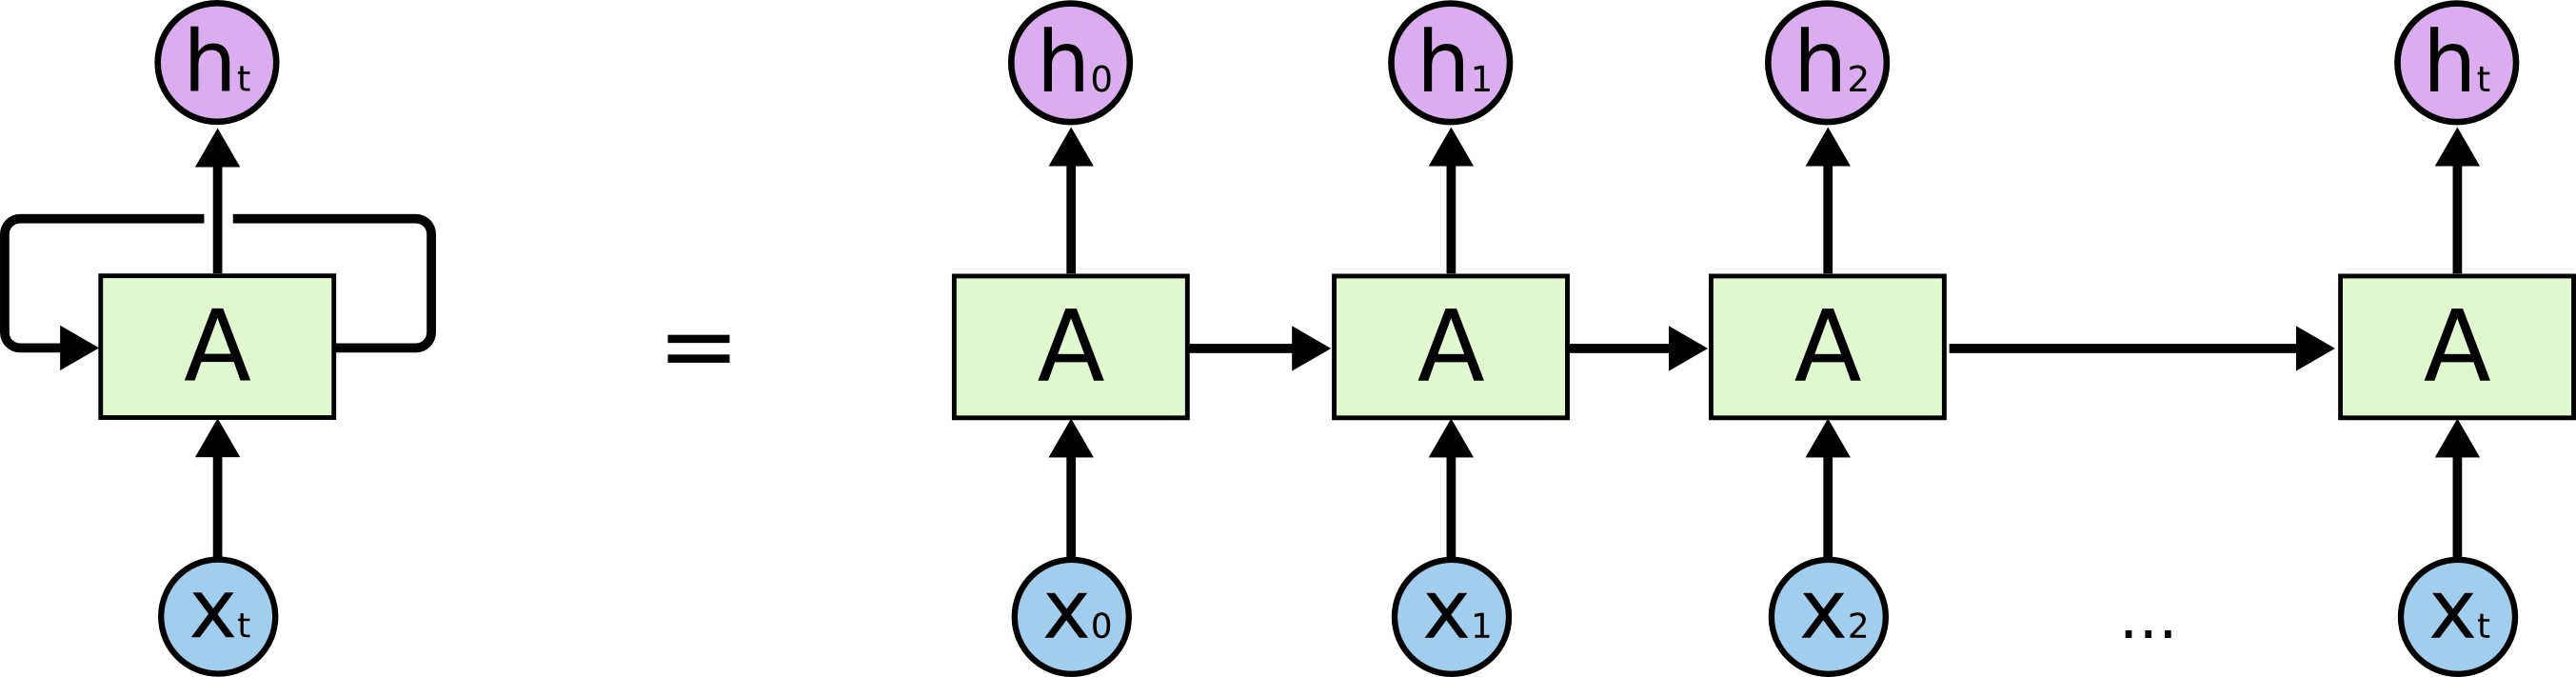
\includegraphics[width=\figureBigSize]
    {figure/model/RNN-unrolled.png}}
    \caption{\label{fig:rnn-unrolled} Recurrent Neural Network đã được trải ra.}
\end{figure}

Bản chất giống như chuỗi này cho thấy các Recurrent neural network có liên quan mật thiết đến các chuỗi và danh sách.
Nó sử dụng kiến trúc tự nhiên của mạng neuron để sử dụng cho dữ liệu đó.

Và chúng chắc chắn được sử dụng!
Trong vài năm qua, đã có những thành công đáng kinh ngạc khi áp dụng RNN cho nhiều vấn đề khác nhau: nhận dạng giọng
nói, mô hình ngôn ngữ, dịch thuật, chú thích hình ảnh.

Điều cần thiết cho những thành công này là việc sử dụng "LSTMs", một loại mạng thần kinh tái phát rất đặc biệt, hoạt
động, cho nhiều tác vụ, tốt hơn nhiều so với phiên bản tiêu chuẩn. Hầu như tất cả các kết quả thú vị dựa trên các mạng thần kinh tái phát đều đạt được với chúng. Nó có những LSTM mà bài tiểu luận này sẽ khám phá.

\textbf{Vấn đề phụ thuộc xa} \\[0.2em]
Một trong những lời kêu gọi của RNN là ý tưởng rằng họ có thể kết nối thông tin trước đó với tác vụ hiện tại, chẳng
hạn như sử dụng các khung video trước đó có thể thông báo cho sự hiểu biết về khung hiện tại. Nếu RNN có thể làm điều
này, thì họ cực kỳ hữu ích. Nhưng họ có thể? Không hẳn.

Đôi khi, chúng ta chỉ cần nhìn vào thông tin gần đây để thực hiện nhiệm vụ hiện tại. Ví dụ, hãy xem xét một mô hình
ngôn ngữ đang cố gắng dự đoán từ tiếp theo dựa trên các từ trước đó. Nếu chúng ta đang cố gắng dự đoán từ cuối cùng
trong "các đám mây trên \textit{bầu trời}", thì chúng ta không cần bất kỳ bối cảnh nào nữa - đó là một điều khá rõ ràng,
từ tiếp theo sẽ là  \textit{bầu trời}. Trong những trường hợp như vậy, khi khoảng cách giữa thông tin liên quan và
địa điểm mà nó cần là nhỏ, RNN có thể học cách sử dụng thông tin trong quá khứ.

\begin{figure}[!htb]
    \center{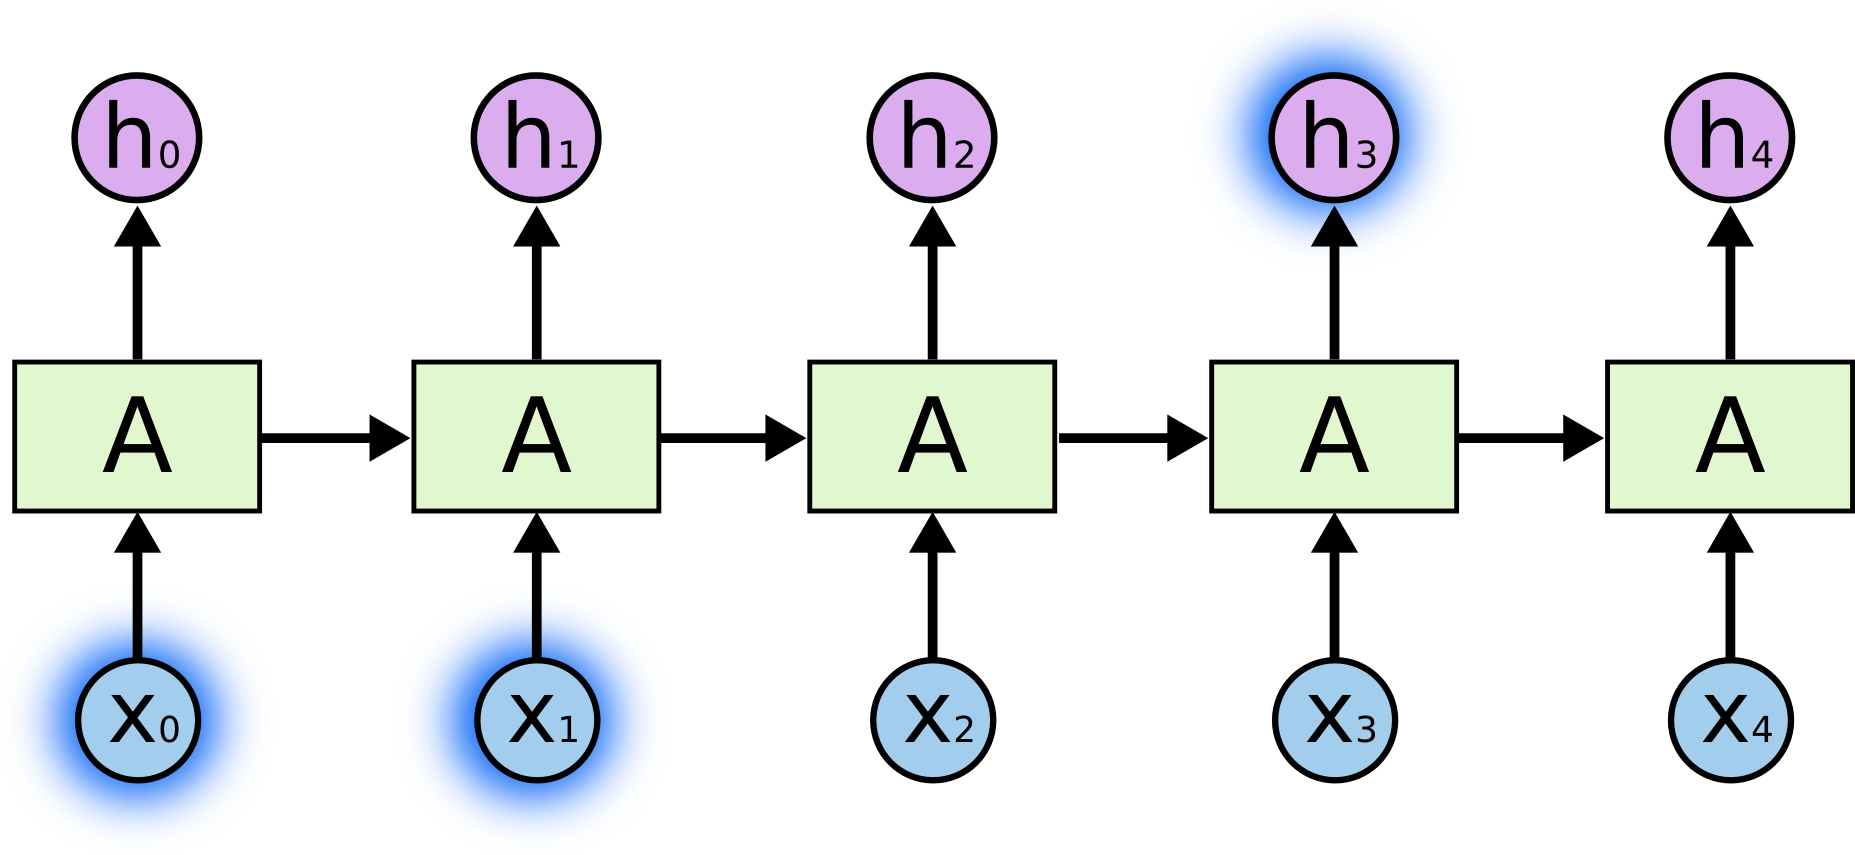
\includegraphics[width=\figureBigSize]
    {figure/model/RNN-shorttermdepdencies.png}}
\end{figure}

Nhưng cũng có những trường hợp chúng ta cần nhiều bối cảnh hơn. Cân nhắc việc cố gắng dự đoán từ cuối cùng trong văn
bản. "Tôi lớn lên ở Việt Nam. Tôi nói tiếng trôi chảy tiếng \textit{Việt}". Thông tin gần đây cho thấy từ tiếp theo có
lẽ là tên của một ngôn ngữ, nhưng nếu chúng ta muốn thu hẹp ngôn ngữ nào, chúng ta cần thu hẹp ngôn ngữ nào bối cảnh
của Việt Nam, từ phía trước. Nó hoàn toàn có thể cho khoảng cách giữa thông tin liên quan và điểm cần thiết để trở
nên rất lớn.

Thật không may, khi khoảng cách đó tăng lên, các RNN trở nên không thể học cách kết nối thông tin.
\begin{figure}[!htb]
    \center{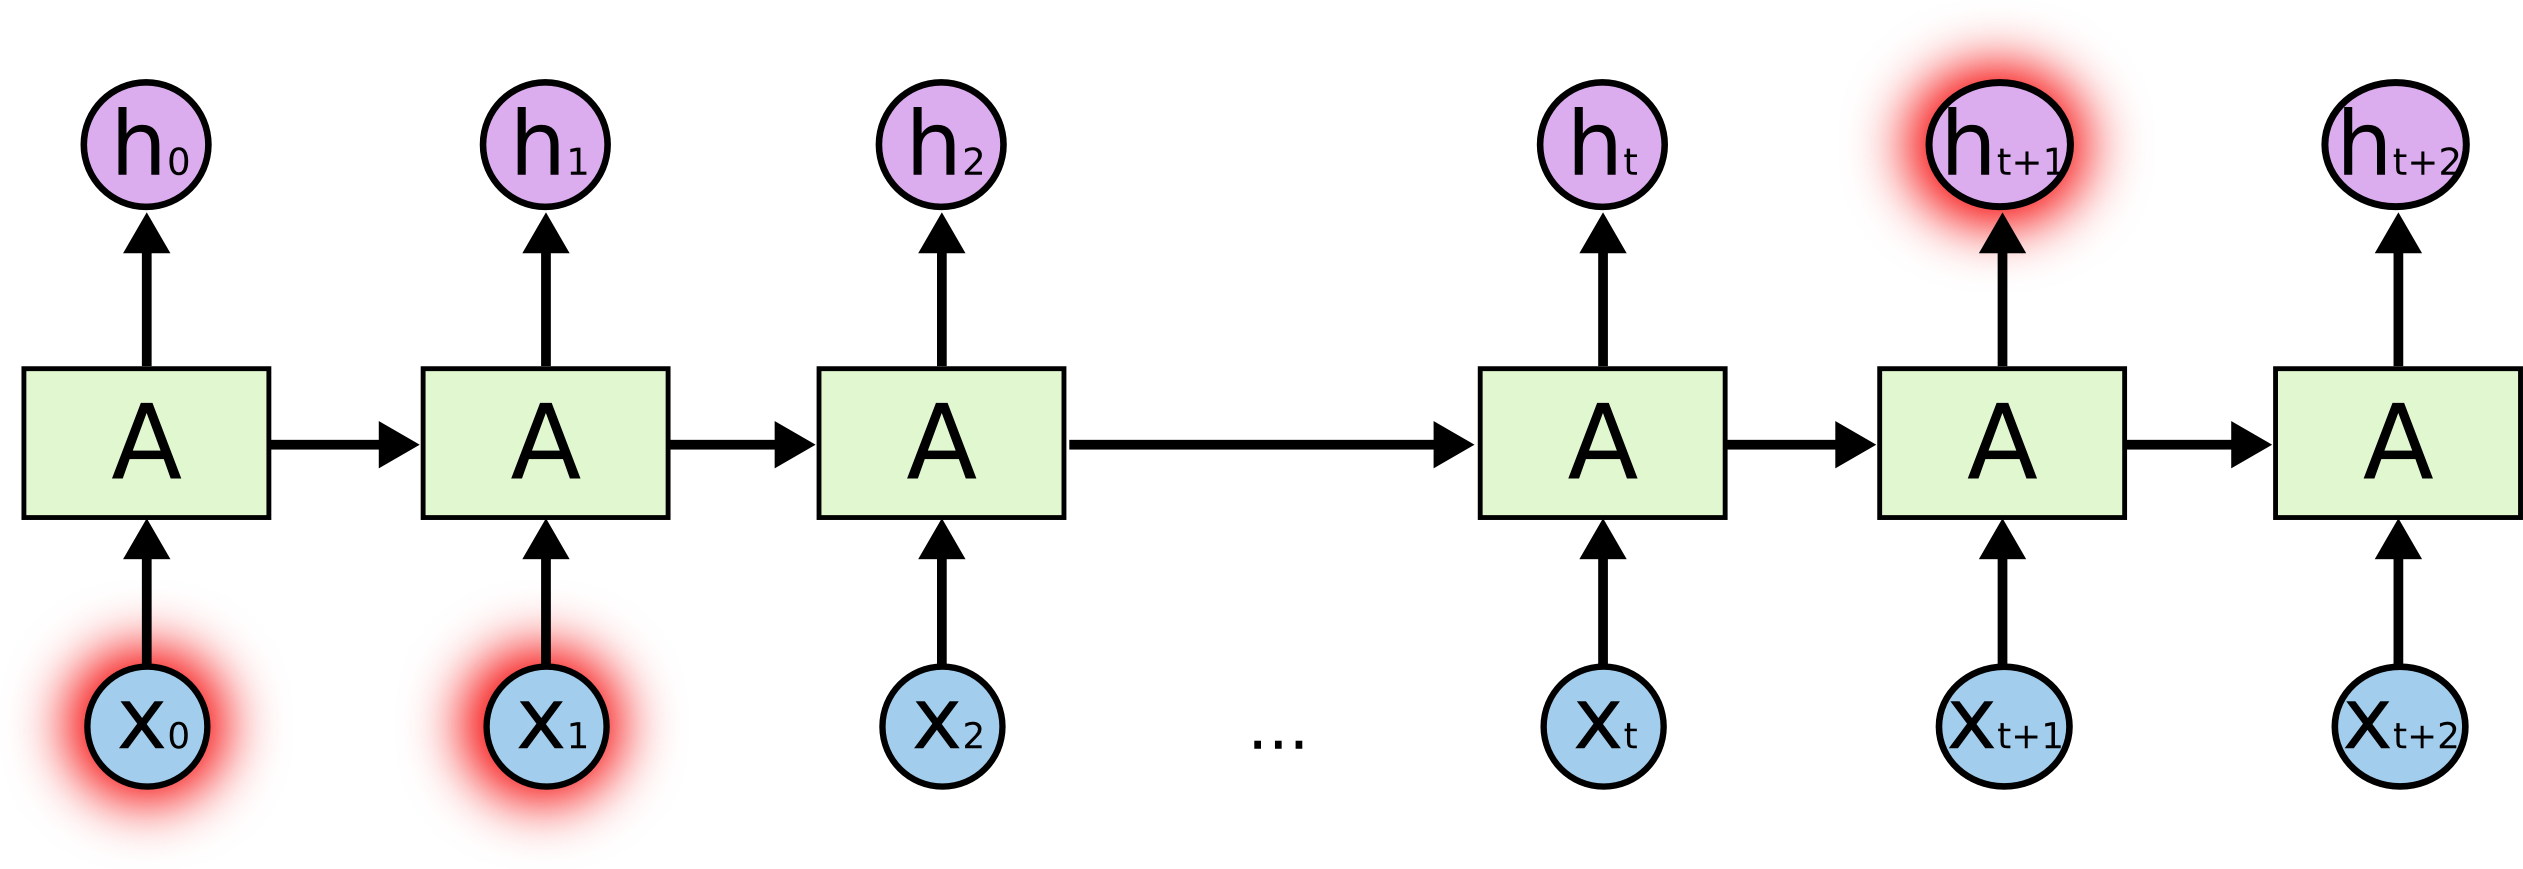
\includegraphics[width=\figureBigSize]
    {figure/model/RNN-longtermdependencies.png}}
\end{figure}


Về lý thuyết, các RNN hoàn toàn có khả năng xử lý các phụ thuộc dài hạn như vậy. Một người có thể cẩn thận chọn các
tham số cho họ để giải quyết các vấn đề về đồ chơi theo hình thức này. Đáng buồn thay, trong thực tế, RNNs don lồng
dường như có thể học chúng. Vấn đề đã được khám phá sâu bởi Hochreiter (1991) [German] và Bengio, et al. (1994),
người đã tìm thấy một số lý do khá cơ bản tại sao nó có thể khó khăn.

Rất may, LSTMs không có vấn đề này!